\documentclass{article}
\usepackage{graphicx} % new way of doing eps files
\usepackage{listings} % nice code layout
\usepackage[usenames]{color} % color
\definecolor{listinggray}{gray}{0.9}
\definecolor{graphgray}{gray}{0.7}
\definecolor{ans}{rgb}{1,0,0}
\definecolor{blue}{rgb}{0,0,1}
% \Verilog{title}{label}{file}
\newcommand{\Verilog}[3]{
  \lstset{language=Verilog}
  \lstset{backgroundcolor=\color{listinggray},rulecolor=\color{blue}}
  \lstset{linewidth=\textwidth}
  \lstset{commentstyle=\textit, stringstyle=\upshape,showspaces=false}
  \lstset{frame=tb}
  \lstinputlisting[caption={#1},label={#2}]{#3}
}


\author{Josh Young}
\title{Lab 2}

\begin{document}
\maketitle

\section{Introduction}
In Lab 2, the user is tasked with testing a MUX and an ADDER by creating a test bench and running a simulation with the MUX and ADDER by feeding it data and observing the output. Vivado was used to create the test bench as well as run the simulation for both the MUX and the ADDER.

\section{Interface}
The inputs for the ADDER are an indentation (i.e. 4) and the signal from the program counter. The output for the ADDER is used to get the next address by using the program counter. The MUX takes the output from the ADDER and feeds an input to the ADDER in order to get an address. The data that these two devices use are in binary.

\section{Design}
Specifically, the MUX and ADDER are used together in order to fetch addresses for instruction memory. There is a kind of feedback loop that connects the MUX and ADDER, where one will update the other.

\section{Implementation}
The code used for creating the MUX can be seen in Listing~\ref{code:reg} on page~\pageref{code:reg}. The code for creating the ADDER can be seen in Listing~\ref{code:adder} on page~\pageref{code:adder}.

\Verilog{Verilog code for implementing a MUX.}{code:reg}{../code/mux.v}

\Verilog{Verilog code for implementing an ADDER.}{code:adder}{../code/adder.v}

\section{Test Bench Design}
The lab had the user create two test benches, one for the MUX, and the other for the ADDER. The goal for the test bench was to try and 'break' the code for the MUX or ADDER. For the ADDER, this was tried by feeding several different numbers to add, I used small and large numbers in decimal where carries would be required. Expected errors would be carry issues, and a potential for overflow. As for the MUX, the test bench was created so that the user could observe how the MUX would operate when feeding inputs, i.e. checking the output change while switching the control wire. The verilog code for the ADDER test bench can be viewed in Listing~\ref{code:addertest} on page~\pageref{code:addertest}, and the code for the MUX test may be viewed in Listing~\ref{code:addertest} on page~\pageref{code:addertest}.

\Verilog{Verilog code for testing an adder.}{code:addertest}{../code/adder_test.v}

\Verilog{Verilog code for testing a mux.}{code:addertest}{../code/mux_test.v}

\section{Simulation}
By viewing the timing diagrams for the MUX and the ADDER, one can see that both behave as expected. The timing diagram for the adder can be viewed in Figure~\ref{fig:regtest}. The timing diagram for the MUX may be viewed in Figure~\ref{fig:muxtest}.



\section{Conclusions}
The goal of this lab was to create test benches for the MUX and ADDER. The purpose of testing these items is to ensure that the code that creates them wont throw errors. Overall, the MUX and ADDER behaved as expected

\begin{figure}
	\begin{center}
		\caption{Timing diagram for the adder test.}\label{fig:regtest}
		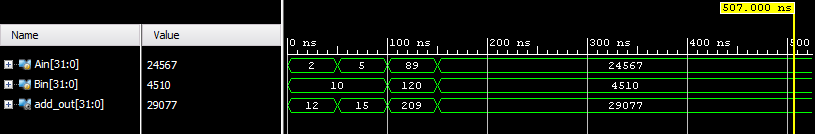
\includegraphics[width=0.9\textwidth]{../images/addertest.png}
	\end{center}
\end{figure}
\begin{figure}
	\begin{center}
		\caption{Timing diagram for the mux test.}\label{fig:muxtest}
		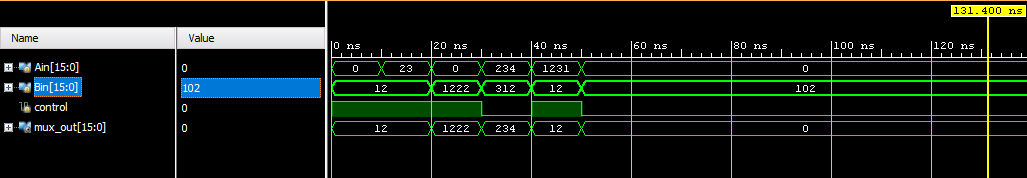
\includegraphics[width=0.9\textwidth]{../images/muxtest.png}
	\end{center}
\end{figure}
\end{document} 
